\documentclass{../../slides-style}

\slidetitle[Лекция 1: Введение в робототехнику]{Алгоритмические основы робототехники}{21.02.2024}

\begin{document}

    \begin{frame}[plain]
        \titlepage
    \end{frame}

    \section{Организационное}

    \begin{frame}
        \frametitle{Организационное}
        \begin{itemize}
            \item Семинары с одной вводной лекцией, две пары в неделю
            \item В конце устный экзамен и аттестация по докладам
            \begin{itemize}
                \item Два вопроса без подготовки
            \end{itemize}
            \item Материалы лекций, темы докладов на \url{https://hwproj.ru}
            \item Балльная система
            \begin{itemize}
                \item 5 баллов за доклад
                \item 10 баллов за экзамен
                \item Итоговая оценка: $(\textrm{<сумма оценок>} -\ 5) * 10$
            \end{itemize}
            \item Коммуникации --- в команде курса в Teams, \url{}
            \begin{itemize}
                \item Также пишите в Teams в личку
            \end{itemize}
        \end{itemize}
    \end{frame}

    \begin{frame}
        \frametitle{Зачем этот курс}
        \begin{itemize}
            \item Робототехника в общем смысле~--- очень перспективна
            \begin{itemize}
                \item Беспилотные автомобили, БПЛА, \enquote{интернет вещей}
            \end{itemize}
            \item Курс~--- краткий обзор того, что вообще бывает, какая наука за этим стоит, чем можно заниматься в магистратуре
            \item Немного общего низкоуровневого программирования, что никогда не лишне
            \item Речь в основном про наземные мобильные роботы
            \item Фокус на алгоритмике:
            \begin{itemize}
                \item Не про паяльники и резьбу по дереву, не про теорию управления, не про искусственный интеллект
            \end{itemize}
            \item Кому нужны робототехники-программисты: \enquote{Сколтех}, ресурсный центр \enquote{Робототехника и БАС} СПбГУ, \enquote{Геоскан}, АО \enquote{Кама}, \enquote{Кибертех}, ЦНИИ РТК, \dots
        \end{itemize}
    \end{frame}

    \begin{frame}
        \frametitle{Что будет в курсе}
        \begin{itemize}
            \item Кинематика мобильного робота: виды и конфигурации колёс, \enquote{стандартная} трёхколёсная тележка, другие варианты кинематики (в т.ч. шагающие роботы)
            \item Сенсорика: типы и физические принципы работы сенсоров, работа с ошибками измерений.
            \item Отдельно видеокамеры, стереокамеры, сенсоры глубины
            \item Алгоритмы машинного зрения, сегментация
            \item Локализация, behavior-driven алгоритмы, belief representation, представление карты
            \item SLAM
            \item Планирование и \enquote{стратегическая} навигация
            \item Аппаратные робототехнические платформы, от Arduino до KUKA
            \item Программные платформы, ROS
        \end{itemize}
    \end{frame}

    \section{Введение}

    \begin{frame}
        \frametitle{Робототехника? Какая робототехника?}
        Робототехника --- наука об автономных технических системах, или о разработке и применении роботов.
        \begin{itemize}
            \item Слово \enquote{Робот} придумал Карел Чапек ещё в 1920
            \item Часто под роботами понимают вообще автоматические машины для замены человека в труде
            \item Следуя традициям СПбГУ, будем понимать под роботами таковые машины \emph{с обратной связью}
            \item Есть ещё \emph{кибернетика} --- наука об управлении, раздел прикладной математики
        \end{itemize}
    \end{frame}

    \begin{frame}
        \frametitle{Какие роботы бывают}
        \begin{columns}
            \begin{column}{0.5\textwidth}
                \begin{itemize}
                    \item Стационарные (манипулятивные) роботы
                    \begin{itemize}
                        \item Промышленные роботы-манипуляторы
                        \item Дельта-роботы
                    \end{itemize}
                    \item Мобильные роботы
                    \begin{itemize}
                        \item Колёсные (гусеничные)
                        \item БПЛА, подводные/надводные
                        \item Шагающие
                    \end{itemize}
                \end{itemize}
            \end{column}
            \begin{column}{0.5\textwidth}
                \begin{center}
                    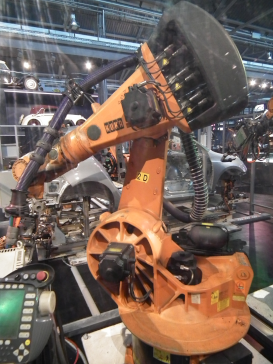
\includegraphics[width=0.4\textwidth]{kuka.png}

                    \vspace{1cm}

                    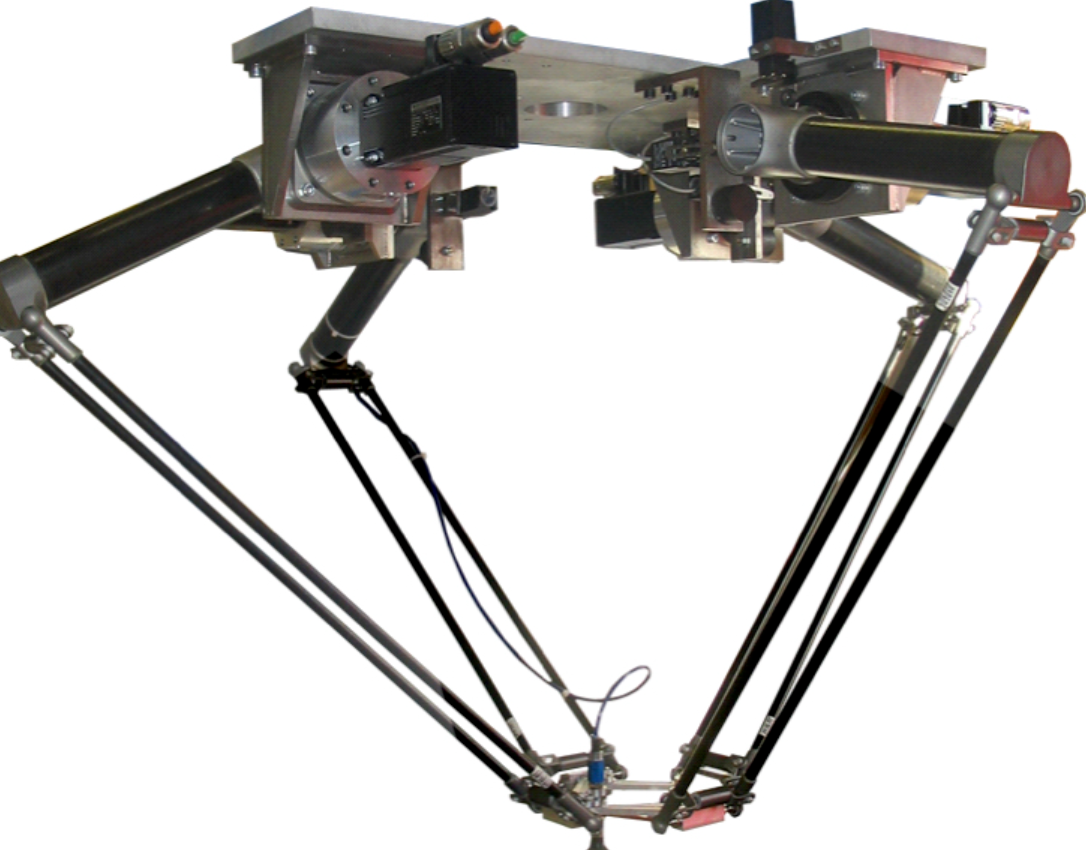
\includegraphics[width=0.5\textwidth]{delta.png}
                \end{center}
            \end{column}
        \end{columns}
    \end{frame}

    \begin{frame}
        \frametitle{Робототехника на матмехе}
        \begin{columns}
            \begin{column}{0.5\textwidth}
                \begin{itemize}
                    \item Образовательный конструктор ТРИК
                    \item Среда программирования TRIK Studio/QReal:Robots
                    \item Ресурсный центр \enquote{Робототехника и БАС}
                    \item Кафедра теоретической кибернетики
                \end{itemize}
            \end{column}
            \begin{column}{0.5\textwidth}
                \begin{center}
                    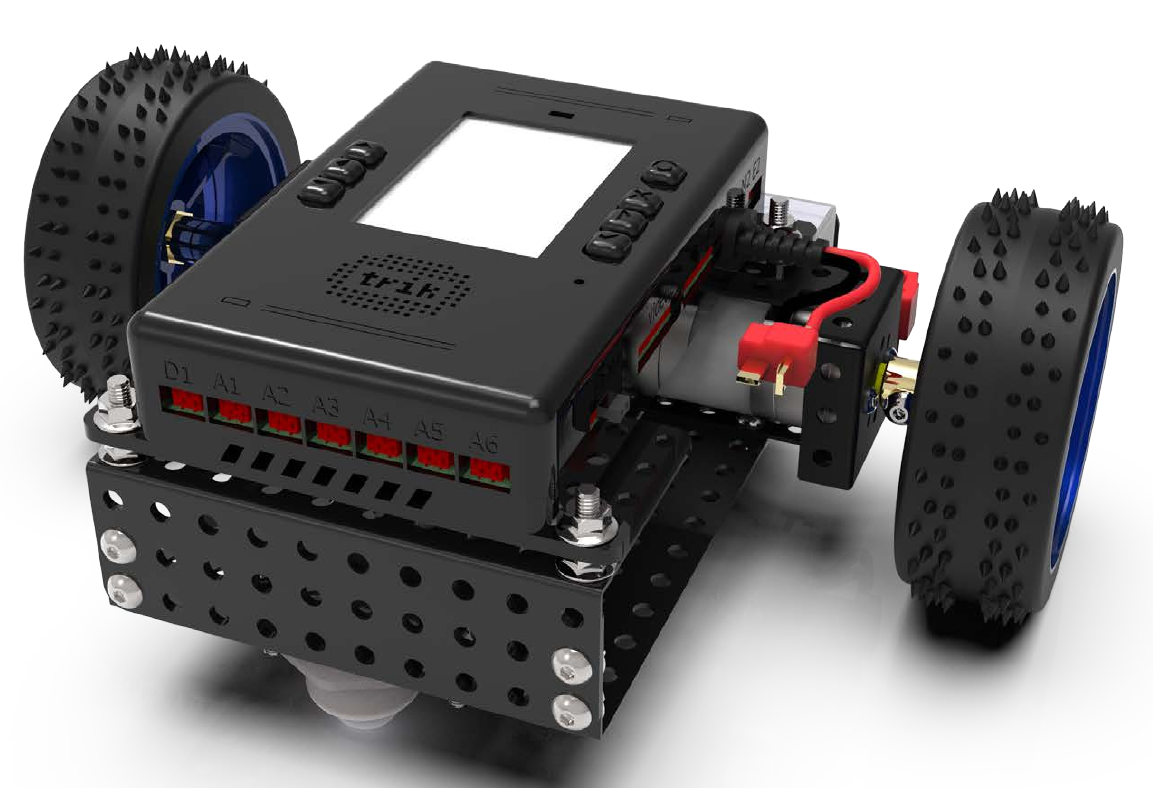
\includegraphics[width=0.6\textwidth]{trik.png}
                \end{center}
            \end{column}
        \end{columns}
    \end{frame}

    \section{Алгоритмические основы}

    \begin{frame}
        \frametitle{Общая схема управления роботом}
        \framesubtitle{Sense-compute-control}
        \begin{center}
            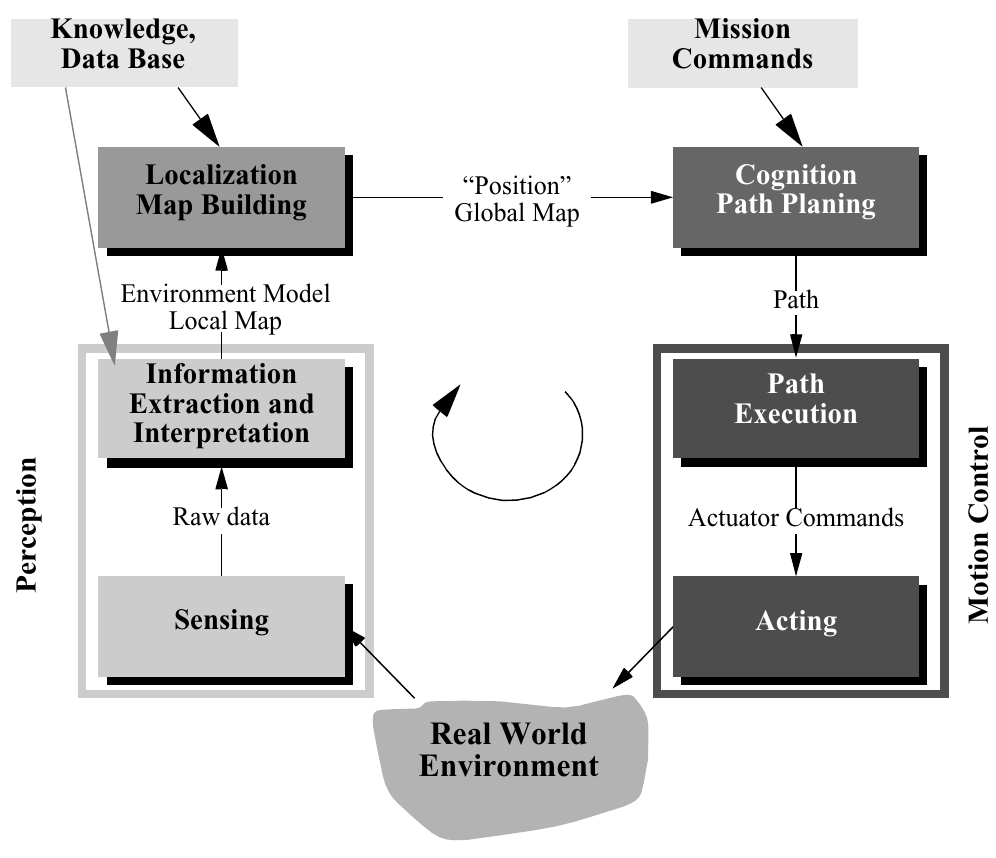
\includegraphics[width=0.6\textwidth]{controlLoop.png}
            \attribution{R. Siegwart, I.R. Nourbakhsh, Introduction to Autonomous Mobile Robots}
        \end{center}
    \end{frame}

    \begin{frame}
        \frametitle{Базовые схемы управления}
        \begin{itemize}
            \item Задача: имея установочное значение, вырабатывать управляющее воздействие так, чтобы система оставалась к установочному значению как можно ближе
            \item Релейный регулятор: скачнообразное переключение управляющего воздействия при достижении порогового значения
            \item Пропорциональный регулятор: управляющее воздействие пропорционально отклонению от установочного значения
            \item Пропорционально-дифференциальный регулятор: управляющее воздействие пропорционально отклонению от установочного значения и скорости отклонения
            \item ПИД-регулятор: управляющее воздействие пропорционально всему выше и длительности отклонения
        \end{itemize}
    \end{frame}

    \begin{frame}
        \frametitle{Демо}
        \begin{center}
            \Huge{Демо на TRIK Studio}
        \end{center}
    \end{frame}

    \begin{frame}
        \frametitle{Продвинутые подходы}
        \begin{columns}
            \begin{column}{0.5\textwidth}
                \begin{itemize}
                    \item Behavior-driven
                    \begin{itemize}
                        \item Условие-реакция
                        \item Конечные автоматы
                        \item Дерево поведений
                    \end{itemize}
                    \item Локализация и планирование
                    \begin{itemize}
                        \item Belief representation
                        \item Представление карты
                        \item Локализация по ориентирам
                        \item SLAM
                    \end{itemize}
                \end{itemize}
            \end{column}
            \begin{column}{0.5\textwidth}
                \begin{center}
                    \includegraphics[width=0.9\textwidth]{slamMap.png}
                    \attribution{\url{https://en.wikipedia.org/wiki/Simultaneous_localization_and_mapping}}
                \end{center}
            \end{column}
        \end{columns}
    \end{frame}

    \section{Кинематика}

    \begin{frame}
        \frametitle{Дьявол кроется в деталях}
        \framesubtitle{Кинематика робота}
        \begin{itemize}
            \item Виды задач
            \begin{itemize}
                \item Прямая кинематическая задача --- есть модель и набор управляющих воздействий, какое положение робот займёт в пространстве?
                \item Обратная кинематическая задача --- есть модель и целевое положение робота, каков набор управляющих воздействий?
            \end{itemize}
            \item Степени свободы --- сколько независимых параметров описывают состояние модели
            \begin{itemize}
                \item Не всегда всеми ими можно управлять
            \end{itemize}
            \item Модели:
            \begin{itemize}
                \item Шагающие --- 2, 4, 6 ног
                \item Колёсные --- четыре известных вида колеса, включая \enquote{шведские} и шар, более десятка известных конфигураций колёсных тележек
                \begin{itemize}
                    \item \enquote{Автомобильное} управление, дифференциальное (\enquote{танковое}), омниколёса, \enquote{Synchro drive}
                \end{itemize}
            \end{itemize}
        \end{itemize}
    \end{frame}

    \begin{frame}
        \frametitle{Пример: синхропривод}
        \begin{center}
            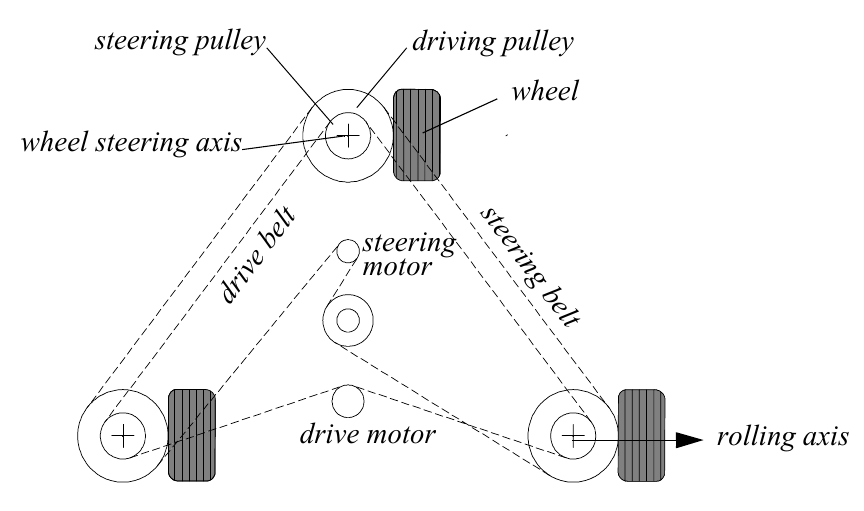
\includegraphics[width=0.7\textwidth]{synchroDrive.png}
            \attribution{R. Siegwart, I.R. Nourbakhsh, Introduction to Autonomous Mobile Robots}
        \end{center}
    \end{frame}

    \begin{frame}
        \frametitle{Поза робота}
        \framesubtitle{Для трёхколёсной дифференциальной тележки}
        \begin{columns}
            \begin{column}{0.6\textwidth}
                \begin{itemize}
                    \item Глобальная система координат
                    \item Поза:
                        $$\xi_I = \begin{bmatrix} x \\ y \\ \theta \end{bmatrix}$$
                    \item Прямая кинематическая модель:
                        $$\dot{\xi_I} = \begin{bmatrix} \dot{x} \\ \dot{y} \\ \dot{\theta} \end{bmatrix} = f(l, r, \theta, \dot{\phi_1}, \dot{\phi_2})$$
                    \item Каждая модель накладывает ограничения на возможные движения
                \end{itemize}
            \end{column}
            \begin{column}{0.4\textwidth}
                \begin{center}
                    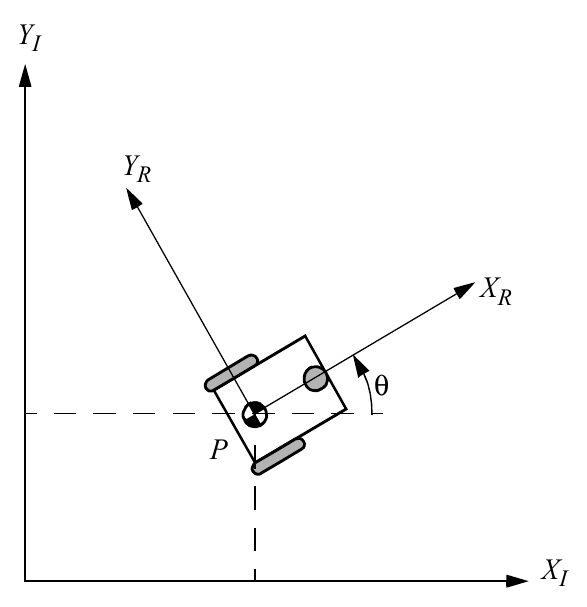
\includegraphics[width=0.8\textwidth]{pose.png}
                    \attribution{R. Siegwart, I.R. Nourbakhsh, Introduction to Autonomous Mobile Robots}
                \end{center}
            \end{column}
        \end{columns}
    \end{frame}

    \begin{frame}
        \frametitle{Задача управления}
        \begin{center}
            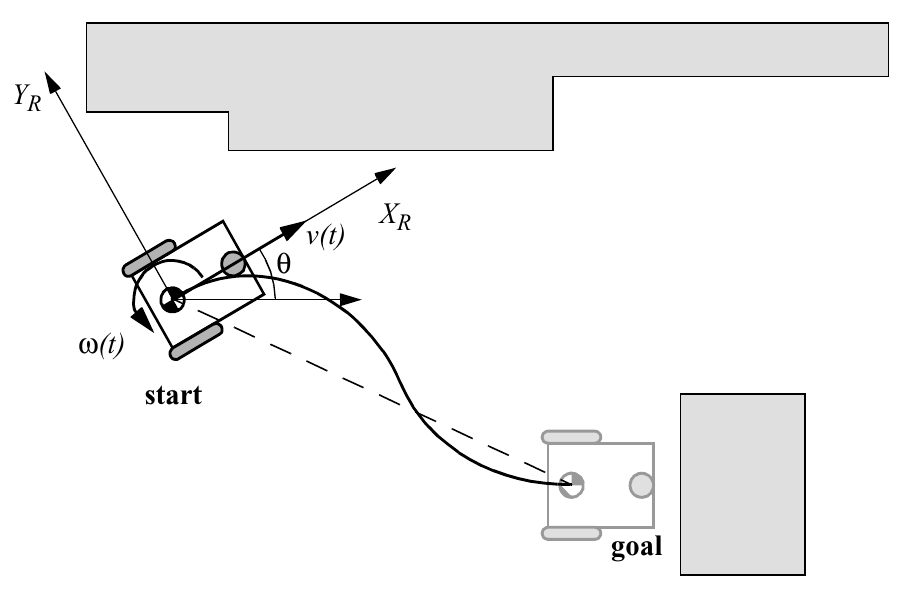
\includegraphics[width=0.7\textwidth]{inverseKinematics.png}
            \attribution{R. Siegwart, I.R. Nourbakhsh, Introduction to Autonomous Mobile Robots}
        \end{center}
    \end{frame}

    \section{Сенсорика}

    \begin{frame}
        \frametitle{Виды сенсоров}
        \begin{itemize}
            \item Тактильные: кнопки, бамперы, неконтактные датчики
            \item Энкодеры, разных видов: оптические, магнитные и т.п.)
            \item Датчики направления: компас, гироскоп, инклинометр
            \item Датчики ориентиров: ГНСС, RF-метки и т.п.
            \item Активные расстояния: УЗ, ИК, лазерные, радар, структурный свет
            \item Движения/скорости: допплеровские радар или звуковые
            \item Машинное зрение: камеры разных видов, стереопары, лидары
        \end{itemize}
    \end{frame}

    \begin{frame}
        \frametitle{Трудности}
        \begin{itemize}
            \item Шумы, фильтрация
            \begin{itemize}
                \item Случайные и систематические ошибки
                \item Фильтр Калмана
            \end{itemize}
            \item Sensor aliasing
            \item Представление неопределённости
            \begin{itemize}
                \item Одна гипотеза, несколько гипотез
            \end{itemize}
            \item Распространение ошибки
            \item Sensor fusion
        \end{itemize}
    \end{frame}

    \begin{frame}
        \frametitle{\enquote{Высокоуровневая} сенсорика}
        \begin{itemize}
            \item Depth from focus
            \item Feature-based-стерео --- много разных алгоритмов сопоставления точек на кадрах с разных ракурсов
            \begin{itemize}
                \item Дескриптор --- некое характерное представление точки, не зависящее от ракурса
            \end{itemize}
            \item Оптический поток (тоже feature-based)
            \item Поиск границ, поиск геометрических примитивов
            \begin{itemize}
                \item Лапласиан гауссиана, преобразование Хафа
            \end{itemize}
            \item Сегментация, кластеризация (сейчас в основном машобуч)
            \begin{itemize}
                \item DBSCAN
            \end{itemize}
            \item Whole-image features --- гистограммы, \enquote{отпечатки}
        \end{itemize}
    \end{frame}

    \begin{frame}
        \frametitle{Общая схема сенсорики на CV}
        \begin{center}
            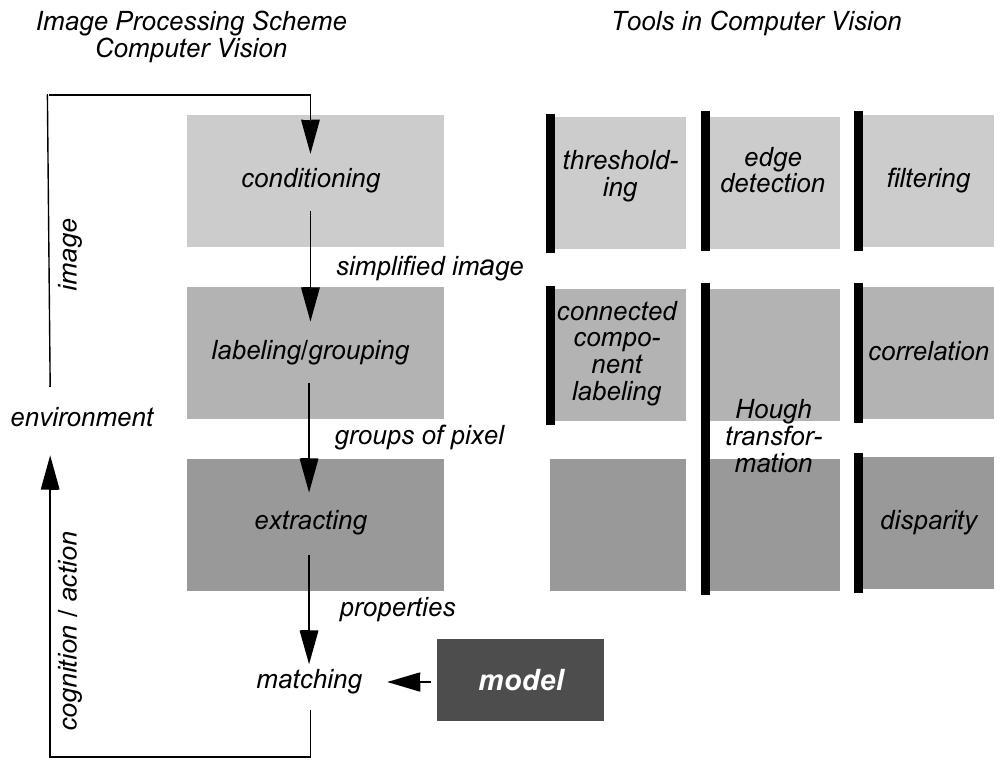
\includegraphics[width=0.7\textwidth]{cvScheme.png}
            \attribution{R. Siegwart, I.R. Nourbakhsh, Introduction to Autonomous Mobile Robots}
        \end{center}
    \end{frame}

    \section{Локализация}

    \begin{frame}
        \frametitle{Задача навигации}
        Behavior-driven-навигация:
        \begin{center}
            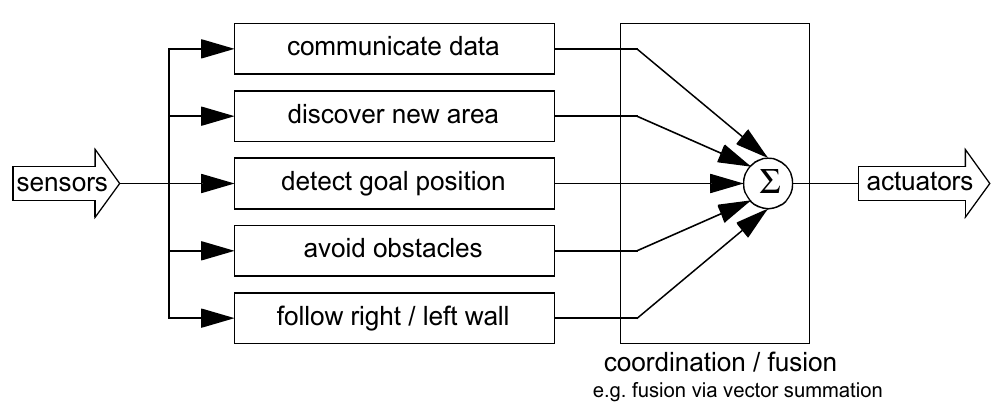
\includegraphics[width=0.5\textwidth]{behaviorNavigation.png}
        \end{center}

        Навигация по карте:
        \begin{center}
            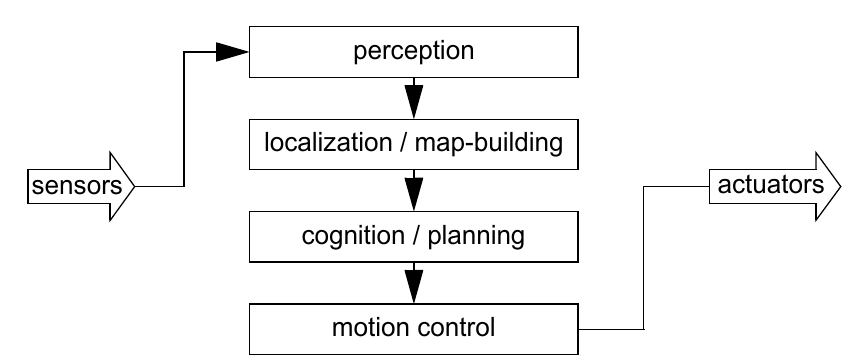
\includegraphics[width=0.5\textwidth]{mapBasedNavigation.png}
            \attribution{R. Siegwart, I.R. Nourbakhsh, Introduction to Autonomous Mobile Robots}
        \end{center}
    \end{frame}

    \begin{frame}
        \frametitle{Определение положения}
        \begin{center}
            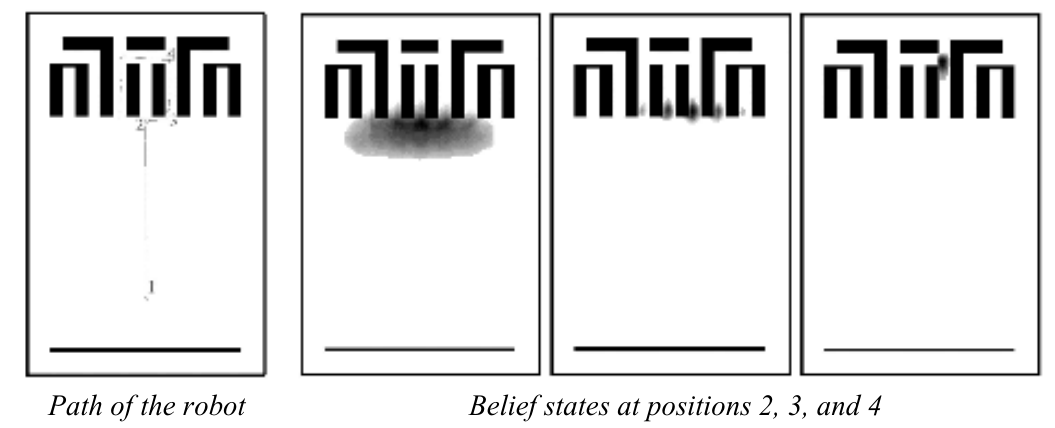
\includegraphics[width=0.9\textwidth]{uncertainity.png}
            \attribution{R. Siegwart, I.R. Nourbakhsh, Introduction to Autonomous Mobile Robots}
        \end{center}
    \end{frame}

    \begin{frame}
        \frametitle{Belief representation}
        \begin{center}
            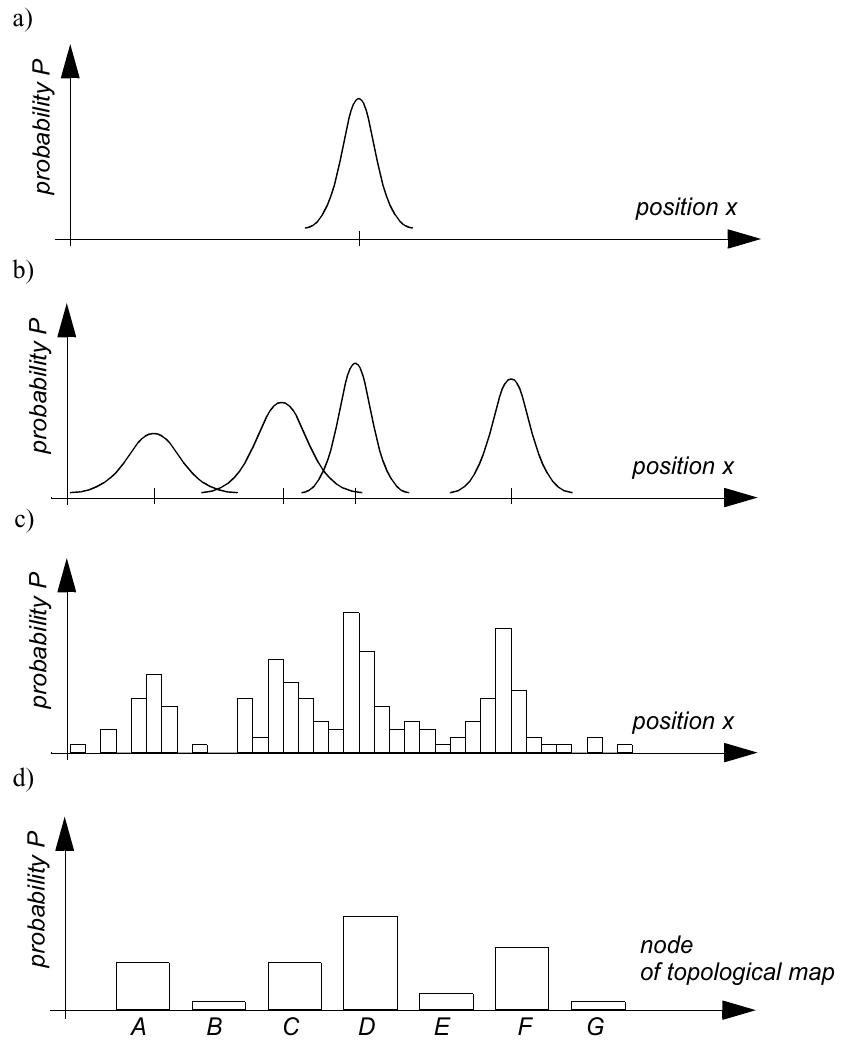
\includegraphics[width=0.45\textwidth]{beliefRepresentation.png}
            \attribution{R. Siegwart, I.R. Nourbakhsh, Introduction to Autonomous Mobile Robots}
        \end{center}
    \end{frame}

    \begin{frame}
        \frametitle{Представление карты}
        \begin{columns}
            \begin{column}{0.5\textwidth}
                \begin{itemize}
                    \item Непрерывное --- геометрические примитивы
                    \item Дискретное:
                    \begin{itemize}
                        \item Сетка
                        \item Сетка с переменным размером ячейки
                        \item Топологическое (в виде графа локаций)
                    \end{itemize}
                \end{itemize}
            \end{column}
            \begin{column}{0.5\textwidth}
                \begin{center}
                    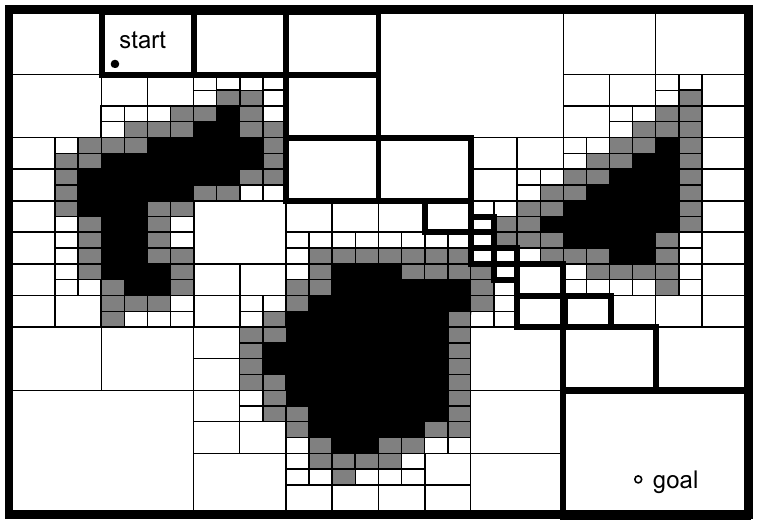
\includegraphics[width=0.8\textwidth]{variableCellGrid.png}
                    \attribution{R. Siegwart, I.R. Nourbakhsh, Introduction to Autonomous Mobile Robots}
                \end{center}
            \end{column}
        \end{columns}
    \end{frame}

    \begin{frame}
        \frametitle{Локализация}
        \begin{itemize}
            \item Инерциальная навигация, проприоцепция
            \item Локализация по ориентирам
            \item Марковская --- поддерживаем набор предположений о том, где мы, уточняем по сенсорам
            \item Фильтр Калмана --- оптимизируем предсказанное положение робота и данные сенсоров
            \item Simultaneous Localization And Mapping --- строим карту и пытаемся определить своё положение на ней
        \end{itemize}
    \end{frame}

    \begin{frame}
        \frametitle{Схема локализации фильтром Калмана}
        \begin{center}
            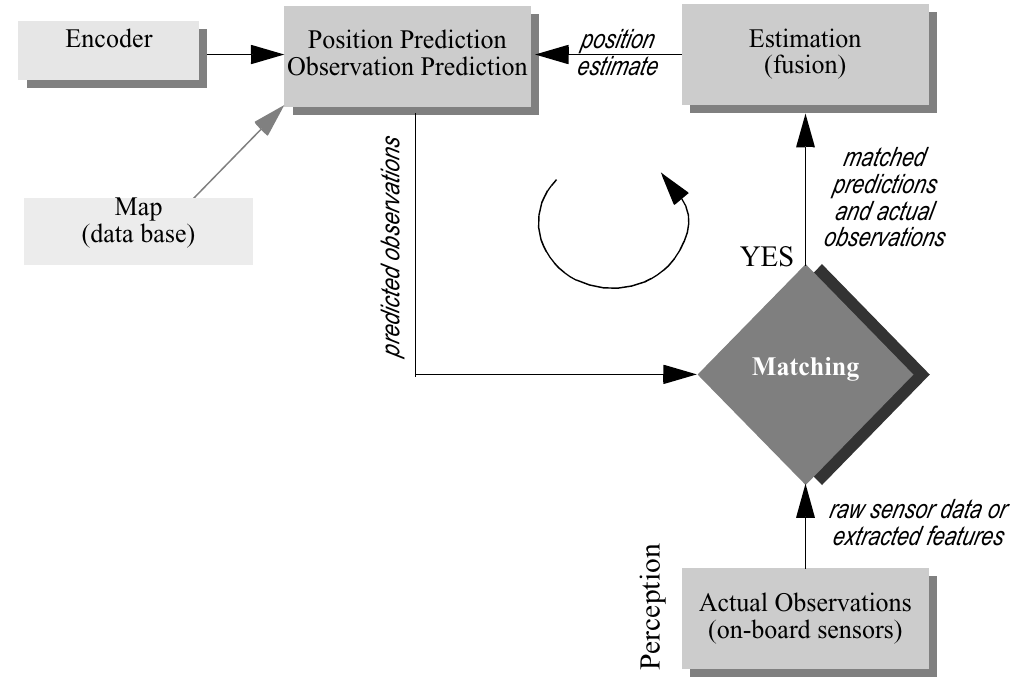
\includegraphics[width=0.6\textwidth]{kalmanLocalization.png}
            \attribution{R. Siegwart, I.R. Nourbakhsh, Introduction to Autonomous Mobile Robots}
        \end{center}
    \end{frame}

    \begin{frame}
        \frametitle{Схема SLAM}
        \begin{center}
            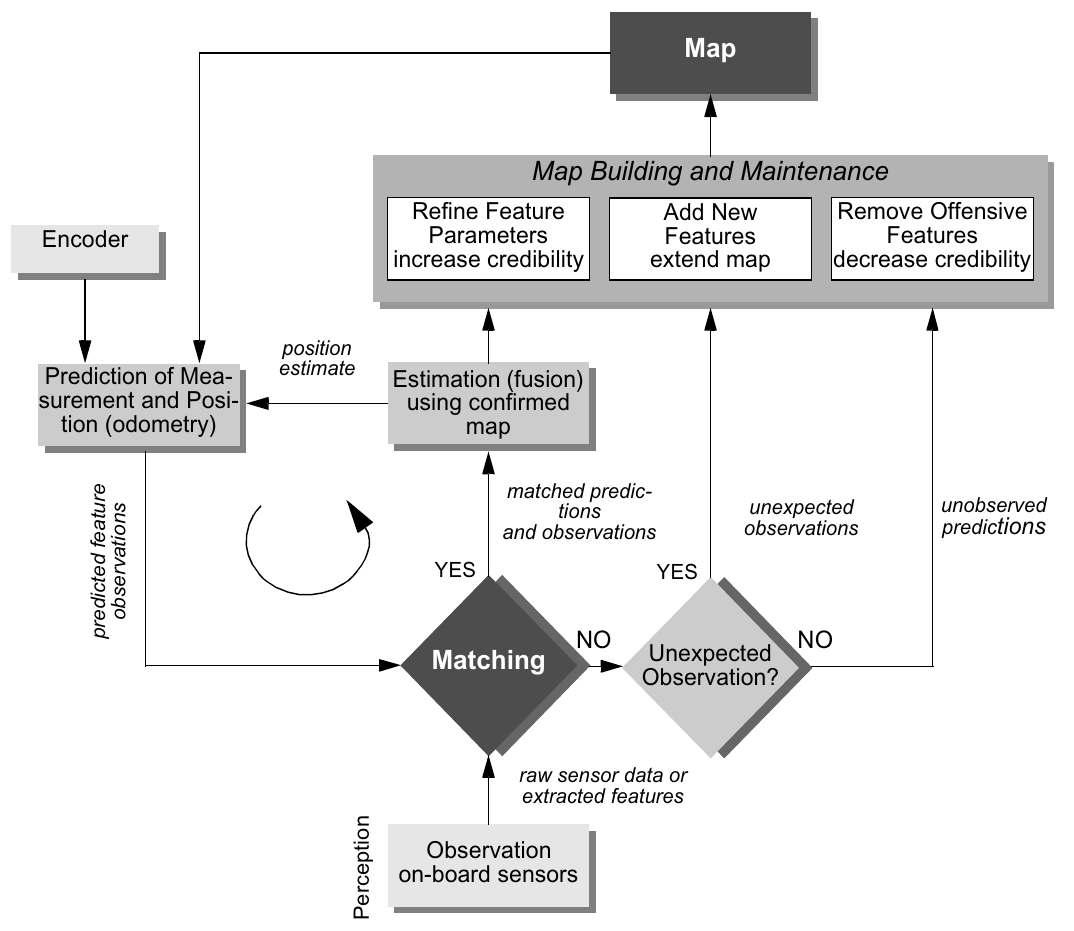
\includegraphics[width=0.65\textwidth]{slam.png}
            \attribution{R. Siegwart, I.R. Nourbakhsh, Introduction to Autonomous Mobile Robots}
        \end{center}
    \end{frame}

    \begin{frame}
        \frametitle{Проблема замыкания траектории}
        \begin{center}
            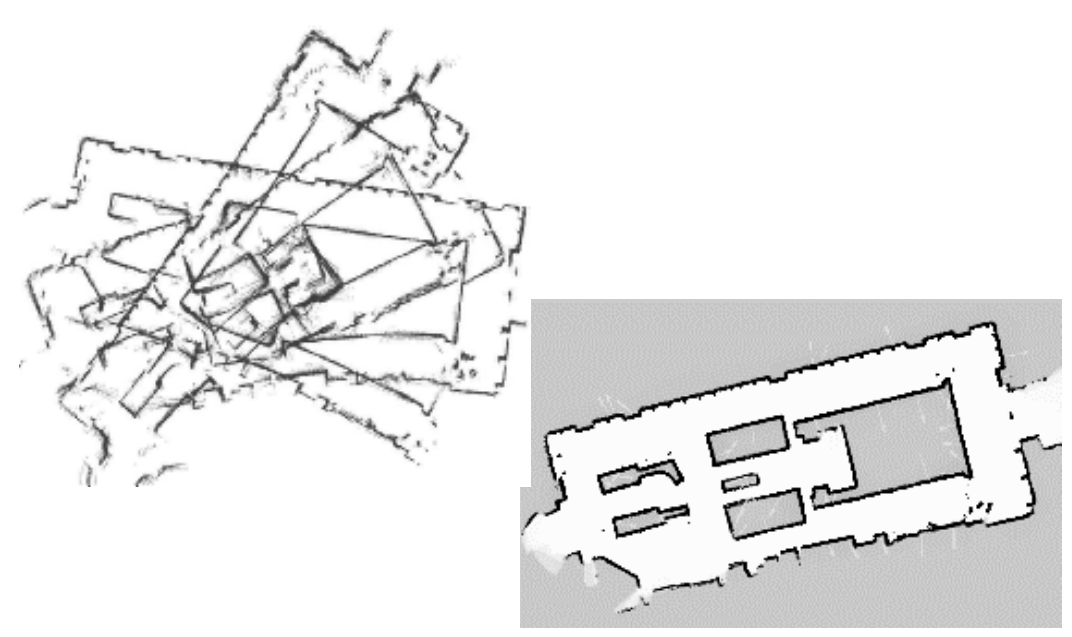
\includegraphics[width=0.7\textwidth]{slamErrors.png}
            \attribution{R. Siegwart, I.R. Nourbakhsh, Introduction to Autonomous Mobile Robots}
        \end{center}
    \end{frame}

    \section{Навигация}

    \begin{frame}
        \frametitle{Задача навигации}
        \begin{itemize}
            \item Задача: зная карту и своё положение на ней, достичь позиции (или группы позиций) $p$ в момент времени не позже $n$
            \item Но есть нюансы:
            \begin{itemize}
                \item Мы достигаем не позиции $p$, а состояния, в котором верим, что достигли позиции $p$, то есть строим траекторию не по карте, а по нашим представлениям
                \item Как правило, мы не знаем точной карты
                \item Карта может меняться со временем
                \begin{itemize}
                    \item Задача обхода препятствий
                \end{itemize}
            \end{itemize}
            \item integrated planning and execution
        \end{itemize}
    \end{frame}

    \begin{frame}
        \frametitle{Слоистая архитектура системы навигации}
        \begin{columns}
            \begin{column}{0.5\textwidth}
                \begin{center}
                    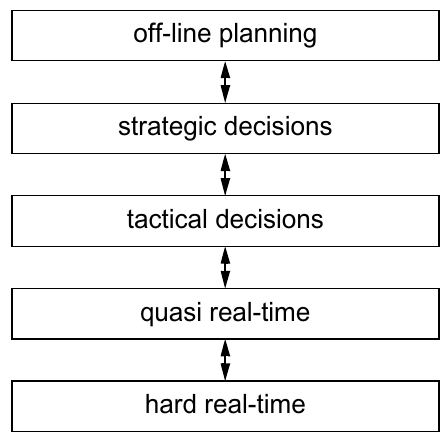
\includegraphics[width=0.7\textwidth]{navigationLayers.png}
                \end{center}
            \end{column}
            \begin{column}{0.5\textwidth}
                \begin{center}
                    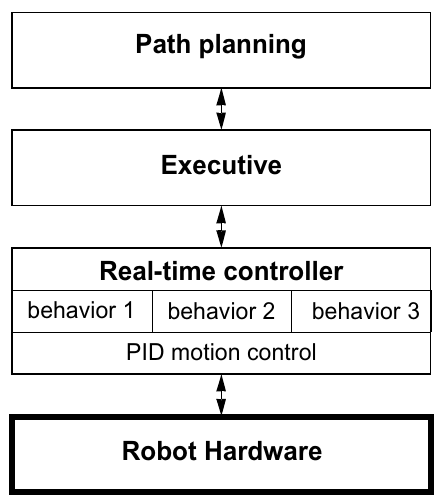
\includegraphics[width=0.7\textwidth]{navigationTiers.png}
                \end{center}
            \end{column}
        \end{columns}
        \attribution{R. Siegwart, I.R. Nourbakhsh, Introduction to Autonomous Mobile Robots}
    \end{frame}

    \section{Программно-инженерные аспекты}

    \begin{frame}
        \frametitle{Аппаратные платформы}
        \begin{columns}
            \begin{column}{0.55\textwidth}
                \begin{itemize}
                    \item Готовые роботы --- KUKA
                    \item Платы \enquote{сделай сам} --- Arduino в различных вариациях, Raspberry Pi, \dots
                    \item Образовательные/платформы для прототипирования --- ТРИК, Vex, Fishertechnik
                \end{itemize}
            \end{column}
            \begin{column}{0.45\textwidth}
                \begin{center}
                    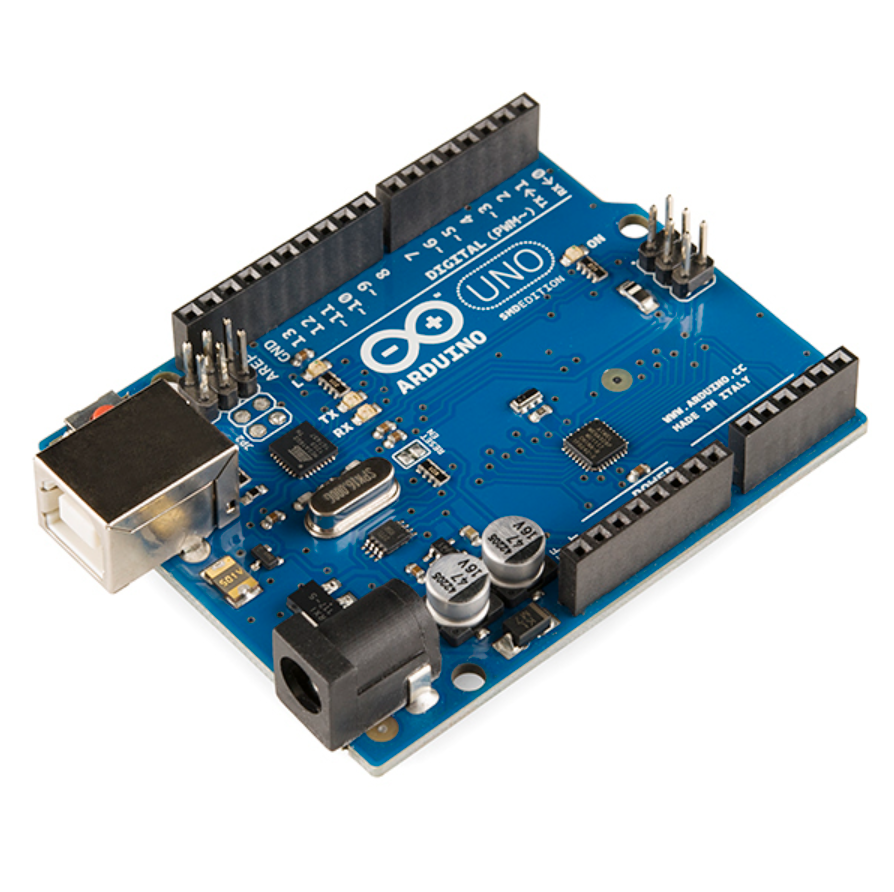
\includegraphics[width=0.6\textwidth]{arduinoUno.png}
                    \attribution{R. Siegwart, I.R. Nourbakhsh, Introduction to Autonomous Mobile Robots}
                \end{center}
            \end{column}
        \end{columns}
    \end{frame}

    \begin{frame}
        \frametitle{Симуляторы}
        \begin{columns}
            \begin{column}{0.5\textwidth}
                \begin{itemize}
                    \item Player/Stage/Gazebo
                    \item Webots
                    \item CoppeliaSim (бывший V-REP)
                    \item Microsoft AirSim
                \end{itemize}
            \end{column}
            \begin{column}{0.5\textwidth}
                \begin{center}
                    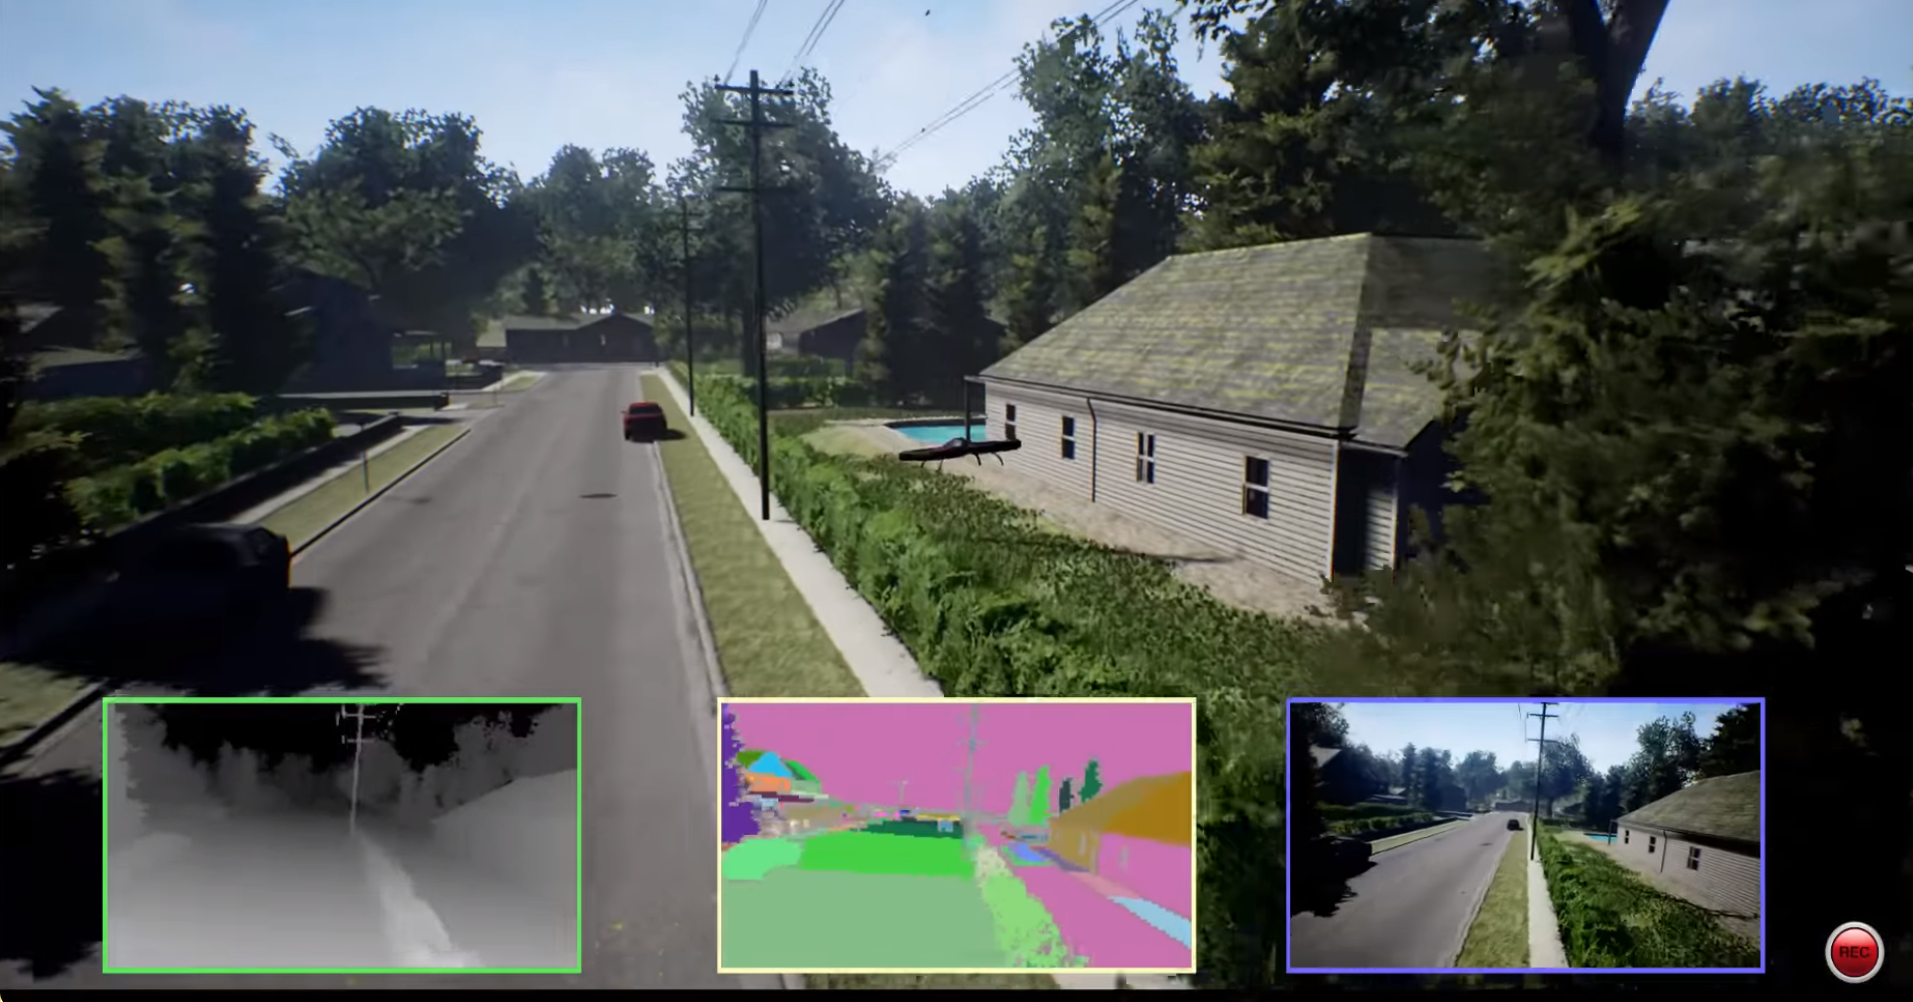
\includegraphics[width=0.8\textwidth]{airSim.png}
                    \attribution{https://microsoft.github.io/AirSim}
                \end{center}
            \end{column}
        \end{columns}
    \end{frame}

    \begin{frame}
        \frametitle{Программные платформы}
        \begin{columns}
            \begin{column}{0.4\textwidth}
                \begin{itemize}
                    \item ROS/ROS2
                    \item Player
                    \item RT-middleware
                    \item YARP
                \end{itemize}
            \end{column}
            \begin{column}{0.6\textwidth}
                \begin{center}
                    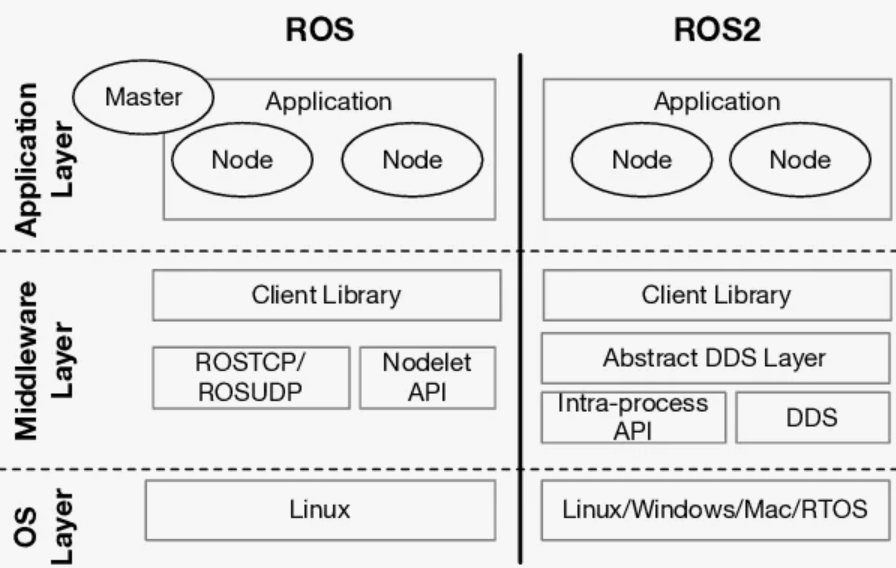
\includegraphics[width=0.9\textwidth]{ros.png}
                    \attribution{\url{https://www.researchgate.net/figure/Comparison-between-ROS-and-ROS2_fig4_335382592}}
                \end{center}
            \end{column}
        \end{columns}
    \end{frame}

    \section{Заключение}

    \begin{frame}
        \frametitle{Книжка}
        \begin{columns}
            \begin{column}{0.5\textwidth}
                Roland Siegwart, Illah Reza Nourbakhsh, Introduction to Autonomous Mobile Robots, MIT Press, 2004, 321 pages
            \end{column}
            \begin{column}{0.5\textwidth}
                \begin{center}
                    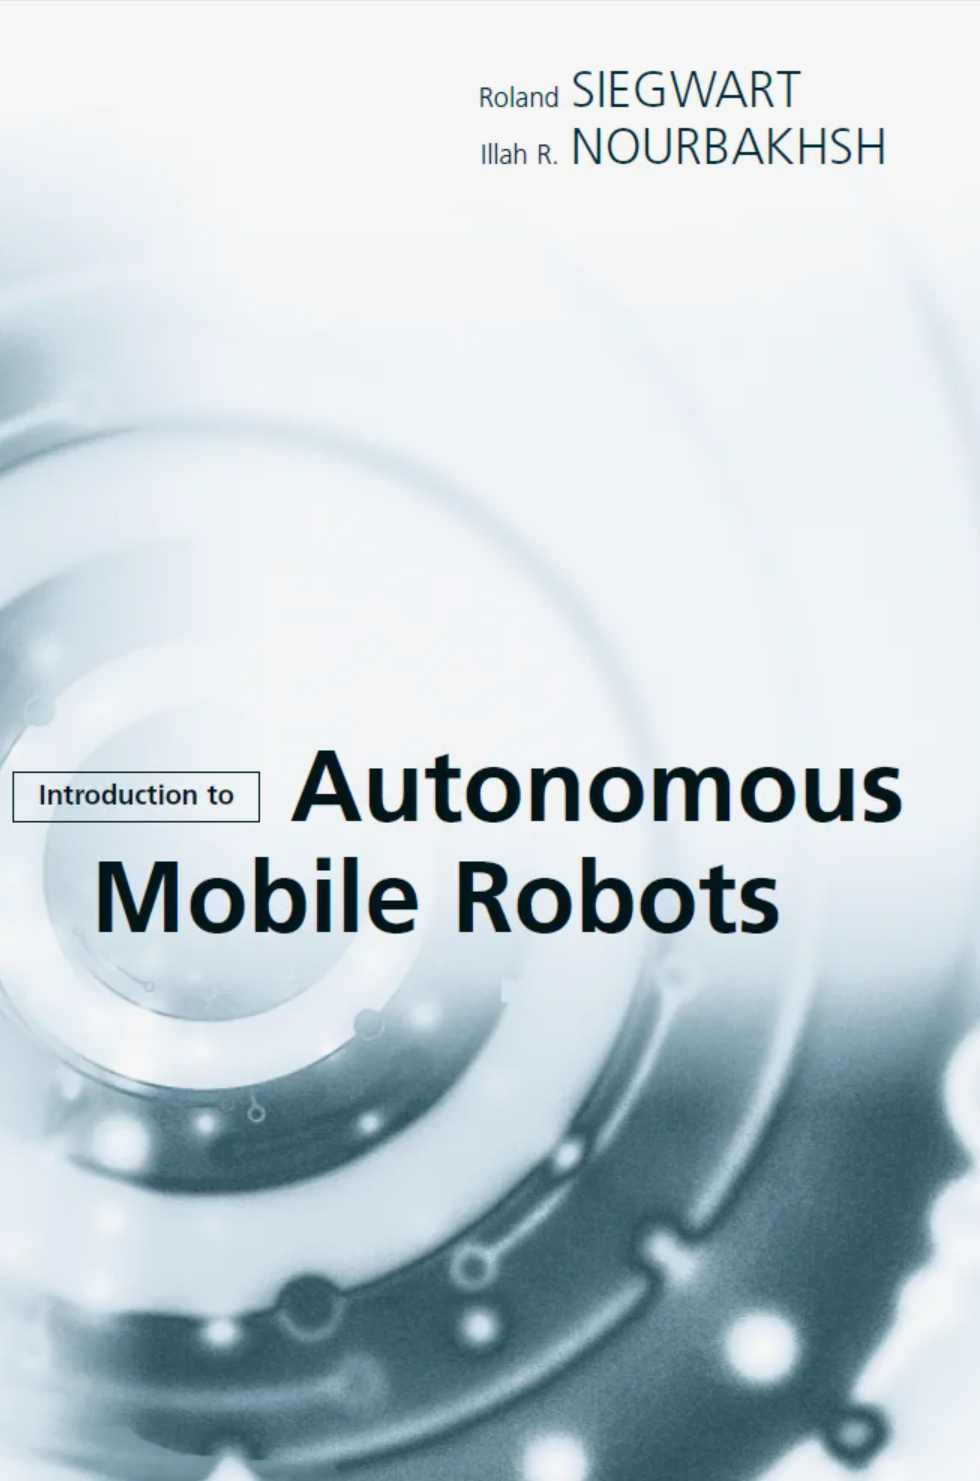
\includegraphics[width=0.7\textwidth]{bookCover.png}
                \end{center}
            \end{column}
        \end{columns}
    \end{frame}

\end{document}
